% 图 55.2 —— 由 `checks/emit_hand.py` 自动拼出（probe 精测 + prims2 图元分解）
%%
% ⚠ 这是**稿子不是成品**：跑 `checks/checkhand.py 55.2` 看指标 + 看叠合图。
%%
%% ⚠ 待核：
%   · 本图 probe 报出阴影族 1 个 —— **本脚本不生成阴影**（要照原书手写）；prims2 的 strokes 里可能含阴影线，核对时留意别画重
%   · 可疑字形 1 项（空心圈 ⊙ 常被认成字母 o）—— 见文件末
%%
\documentclass[12pt]{standalone}
\usepackage{fontspec}
\setsansfont{Arial}
\newfontfamily\mfallback{DejaVu Sans}
\usepackage{tikz}
\begin{document}
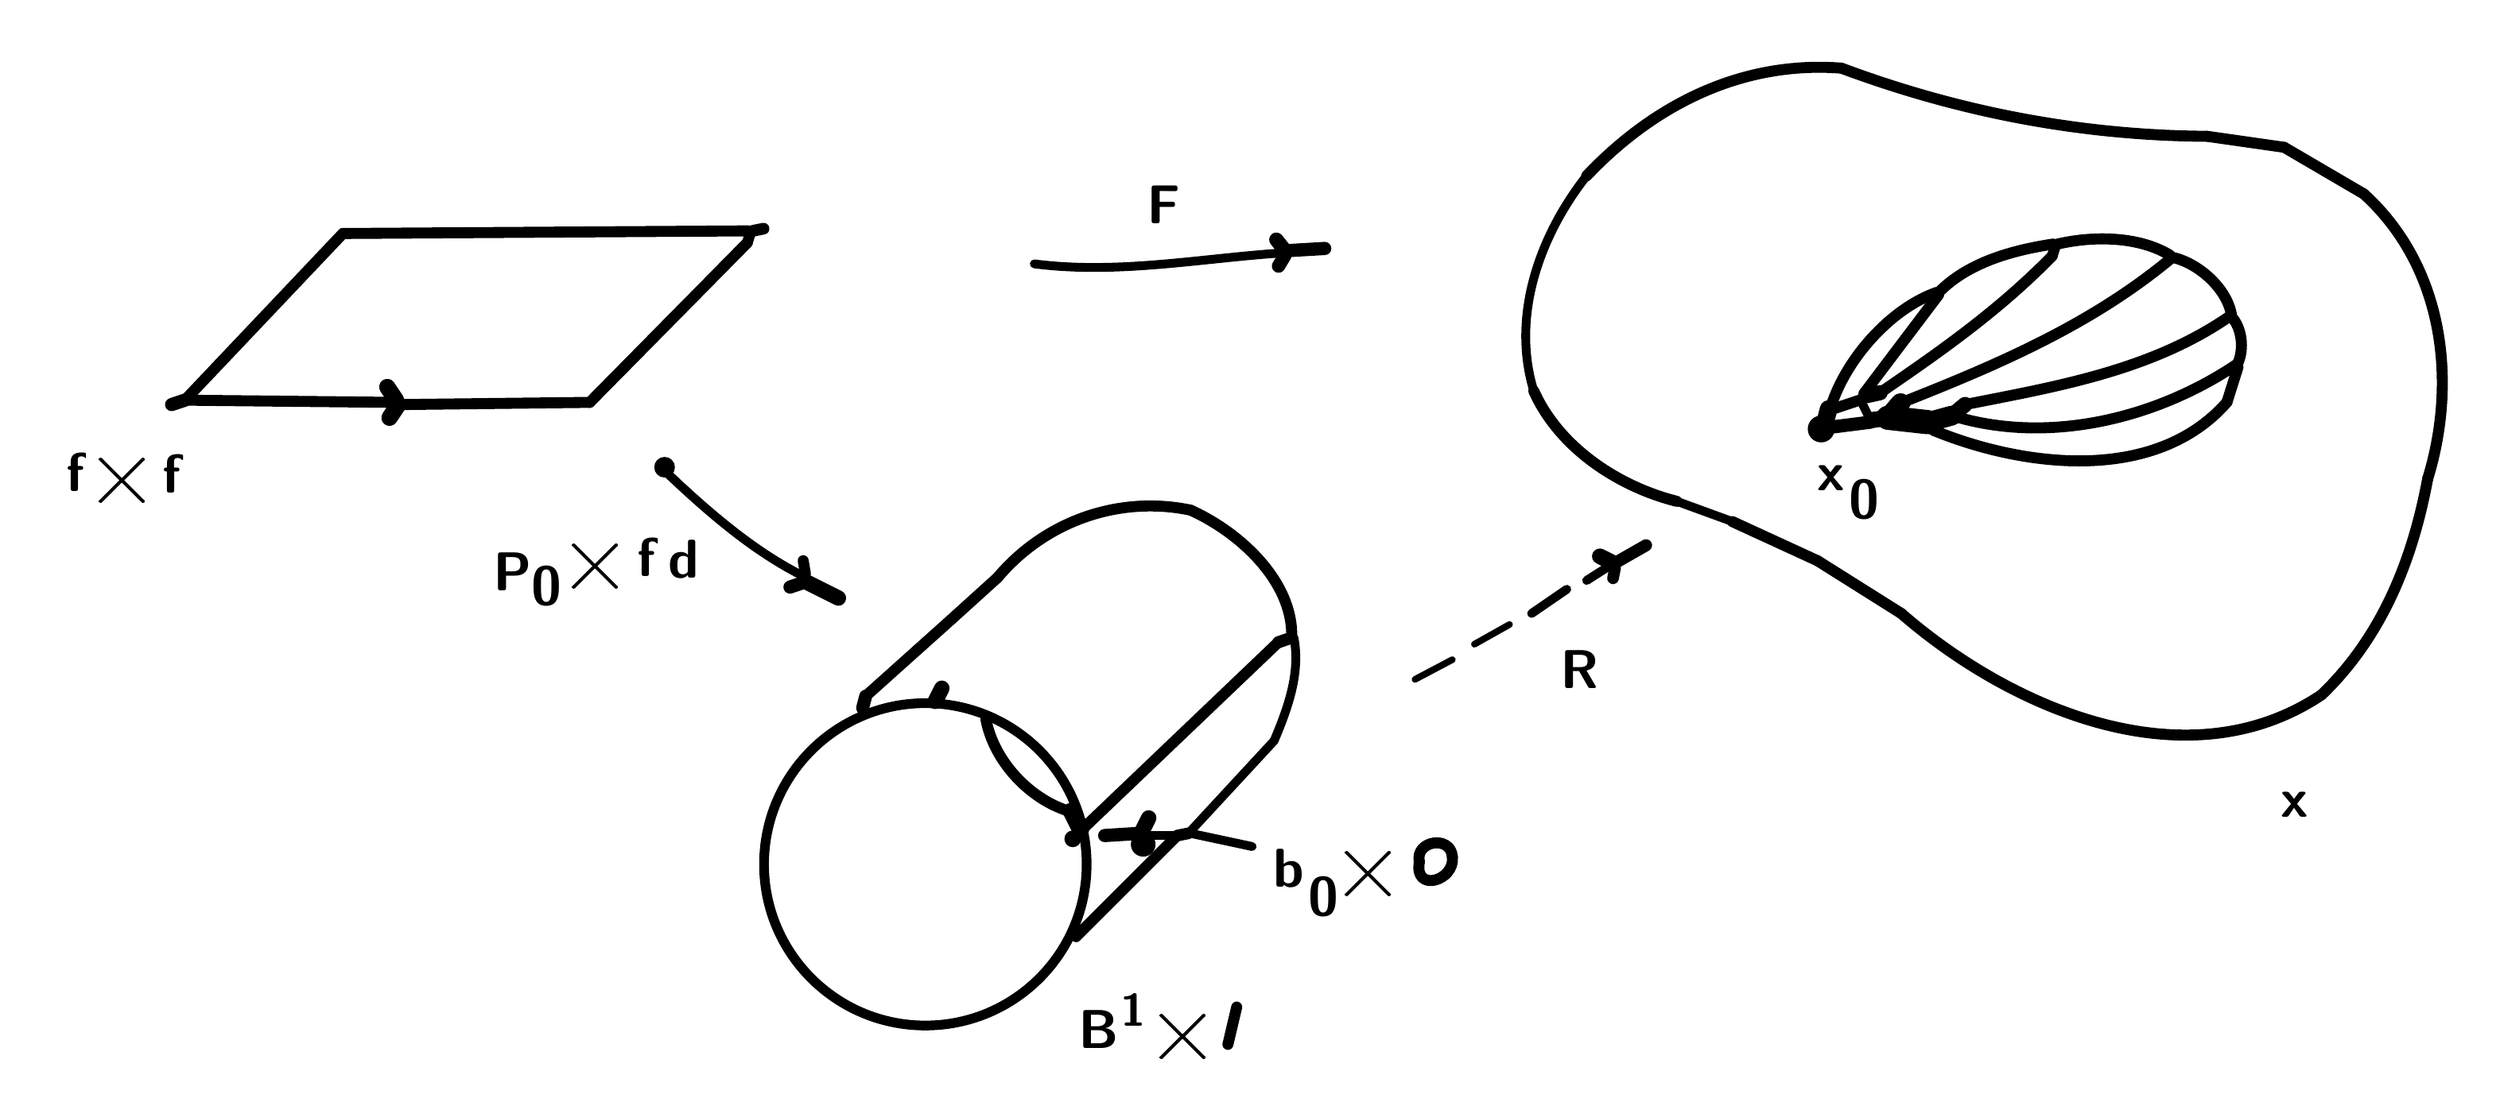
\begin{tikzpicture}[x=1pt, y=-1pt, line width=4.4pt, line cap=round, line join=round]

  %% ════ 填充区（prims2 的 fills）════

  %% ════ 直线段（prims2 的 strokes）════
  \draw[line width=5.0pt] (355.0,245.0) -- (356.0,251.0);
  \draw[line width=7.0pt] (357.0,255.0) -- (371.0,262.0);
  \draw[line width=5.0pt] (823.0,176.0) -- (835.0,172.0);
  \draw[line width=4.0pt] (569.0,326.9) -- (531.0,368.0);
  \draw[line width=8.9pt] (848.0,180.0) -- (853.7,173.3);
  \draw[line width=7.3pt] (848.0,180.0) -- (841.0,181.0);
  \draw[line width=11.0pt] (848.0,180.0) -- (866.0,182.0);
  \draw[line width=4.0pt] (559.0,375.0) -- (531.0,369.0);
  \draw[line width=5.0pt] (552.0,448.0) -- (548.0,465.0);
  \draw[line width=7.0pt] (415.0,309.0) -- (418.0,303.0);
  \draw[line width=6.0pt] (508.0,369.0) -- (492.0,370.0);
  \draw[line width=7.4pt] (171.0,174.0) -- (167.0,180.0);
  \draw[line width=3.0pt] (676.0,274.0) -- (660.0,283.0);
  \draw[line width=5.5pt] (724.0,246.0) -- (738.0,238.0);
  \draw[line width=6.0pt] (840.0,182.0) -- (818.7,184.7);
  \draw[line width=8.0pt] (818.7,184.7) -- (821.0,176.0);
  \draw[line width=4.0pt] (512.0,370.0) -- (524.0,370.0);
  \draw[line width=3.0pt] (650.0,290.0) -- (633.0,299.0);
  \draw[line width=6.5pt] (570.0,99.0) -- (574.0,104.0);
  \draw[line width=7.0pt] (883.0,174.0) -- (877.0,179.0);
  \draw[line width=5.0pt] (1007.0,157.0) -- (1002.0,172.9);
  \draw[line width=4.9pt] (868.8,185.8) -- (866.0,182.0);
  \draw[line width=5.0pt] (74.0,172.0) -- (145.8,96.2);
  \draw[line width=5.0pt] (145.8,96.2) -- (330.0,95.0);
  \draw[line width=6.0pt] (74.0,172.0) -- (68.0,174.0);
  \draw[line width=5.0pt] (74.0,172.0) -- (169.0,173.0);
  \draw[line width=8.0pt] (481.0,367.0) -- (477.0,359.0);
  \draw[line width=4.0pt] (702.0,258.0) -- (686.0,269.0);
  \draw[line width=7.0pt] (512.0,362.0) -- (509.0,368.0);
  \draw[line width=6.0pt] (349.0,257.0) -- (355.0,255.0);
  \draw[line width=5.0pt] (524.0,371.0) -- (479.0,416.0);
  \draw[line width=5.0pt] (837.0,169.0) -- (871.0,124.0);
  \draw[line width=5.3pt] (525.0,370.0) -- (530.0,369.0);
  \draw[line width=4.0pt] (722.0,247.0) -- (711.0,254.0);
  \draw[line width=6.9pt] (838.0,170.0) -- (844.4,168.6);
  \draw[line width=4.9pt] (922.6,106.4) -- (924.0,102.0);
  \draw[line width=7.4pt] (166.0,166.0) -- (170.0,172.0);
  \draw[line width=9.0pt] (877.0,179.0) -- (866.0,182.0);
  \draw[line width=7.1pt] (723.0,246.0) -- (717.0,243.0);
  \draw[line width=4.0pt] (836.0,173.0) -- (840.0,181.0);
  \draw[line width=6.0pt] (575.0,104.0) -- (592.0,103.0);
  \draw[line width=6.1pt] (571.0,111.0) -- (574.0,106.0);
  \draw[line width=5.5pt] (577.0,280.0) -- (570.9,282.1);
  \draw[line width=5.0pt] (570.9,282.1) -- (482.0,367.0);
  \draw[line width=4.9pt] (331.0,96.0) -- (329.6,100.4);
  \draw[line width=5.0pt] (329.6,100.4) -- (258.0,173.0);
  \draw[line width=5.0pt] (258.0,173.0) -- (172.0,174.0);
  \draw[line width=5.3pt] (332.0,95.0) -- (337.0,94.0);
  \draw[line width=5.3pt] (723.0,253.0) -- (724.0,248.0);
  \draw[line width=5.9pt] (382.0,312.0) -- (383.4,306.6);
  \draw[line width=5.0pt] (383.4,306.6) -- (422.1,271.9);
  \draw[line width=5.0pt] (422.1,271.9) -- (443.3,252.7);
  \draw[line width=5.0pt] (993.0,52.0) -- (1028.0,57.0);
  \draw[line width=5.0pt] (1028.0,57.0) -- (1064.2,78.2);
  \draw[line width=5.0pt] (854.0,269.0) -- (815.9,245.0);
  \draw[line width=5.0pt] (815.9,245.0) -- (777.2,227.2);
  \draw[line width=4.0pt] (777.2,227.2) -- (752.0,218.0);

  %% ════ 曲线（prims2 的 curves —— 三段式，坐标同为 (y,x)）════
  \draw[line width=4.0pt] (578.0,280.0) .. controls (581.1,296.3) and (575.1,312.4) .. (569.0,326.9);
  \draw[line width=5.0pt] (853.7,173.3) .. controls (896.5,156.4) and (939.5,138.2) .. (976.0,108.0);
  \draw[line width=4.0pt] (573.0,105.0) .. controls (535.5,107.5) and (497.9,114.9) .. (460.0,110.0);
  \draw[line width=5.0pt] (870.0,123.0) .. controls (848.6,130.7) and (828.8,153.5) .. (822.0,175.0);
  \draw[line width=4.0pt] (355.0,252.0) .. controls (332.3,240.6) and (312.1,223.1) .. (293.0,205.0);
  \draw[line width=5.0pt] (1006.0,156.0) .. controls (969.3,180.6) and (920.3,192.4) .. (877.0,179.0);
  \draw[line width=5.0pt] (1003.0,134.0) .. controls (967.3,158.6) and (924.5,165.8) .. (883.0,174.0);
  \draw[line width=5.0pt] (1002.0,172.9) .. controls (969.5,210.1) and (909.6,202.5) .. (868.8,185.8);
  \draw[line width=5.0pt] (844.4,168.6) .. controls (872.0,149.7) and (898.4,131.2) .. (922.6,106.4);
  \draw[line width=5.0pt] (438.0,317.0) .. controls (441.5,335.9) and (457.6,353.4) .. (476.0,359.0);
  \draw[line width=5.0pt] (1007.0,155.0) .. controls (1009.8,148.8) and (1008.9,139.2) .. (1004.0,134.0);
  \draw[line width=5.0pt] (1004.0,133.0) .. controls (1001.8,120.8) and (988.6,109.4) .. (977.0,107.0);
  \draw[line width=5.0pt] (923.0,101.0) .. controls (904.5,103.8) and (884.2,109.4) .. (871.0,123.0);
  \draw[line width=5.0pt] (925.0,101.0) .. controls (941.3,97.2) and (961.8,97.4) .. (976.0,106.0);
  \draw[line width=5.0pt] (443.3,252.7) .. controls (464.9,227.0) and (498.5,215.2) .. (531.0,222.0);
  \draw[line width=5.0pt] (531.0,222.0) .. controls (553.2,232.0) and (577.1,253.9) .. (577.0,279.0);
  \draw[line width=5.0pt] (711.0,70.0) .. controls (741.7,37.5) and (781.7,17.5) .. (826.8,21.0);
  \draw[line width=5.0pt] (826.8,21.0) .. controls (879.3,40.6) and (934.5,51.6) .. (993.0,52.0);
  \draw[line width=5.0pt] (1064.2,78.2) .. controls (1100.7,111.4) and (1106.8,163.6) .. (1093.2,207.8);
  \draw[line width=5.0pt] (1093.2,207.8) .. controls (1086.5,244.0) and (1072.8,279.3) .. (1045.0,306.0);
  \draw[line width=5.0pt] (1045.0,306.0) .. controls (984.2,346.8) and (904.3,312.8) .. (854.0,269.0);
  \draw[line width=5.0pt] (752.0,218.0) .. controls (725.7,211.4) and (698.6,193.8) .. (687.0,167.8);
  \draw[line width=4.0pt] (687.0,167.8) .. controls (676.5,133.6) and (689.8,96.9) .. (711.0,70.0);
  \draw[line width=5.0pt] (635.0,382.0) .. controls (632.8,372.3) and (649.3,369.6) .. (650.0,379.7);
  \draw[line width=5.0pt] (650.0,379.7) .. controls (651.3,390.6) and (632.4,396.2) .. (635.0,382.0);

  %% ════ 圆 / 椭圆（probe 精测）════
  \draw (410.5,383.1) circle (73.3);

  %% ════ 实心点 ════
  \fill (817.6,185.1) circle (6.1);
  \fill (292.0,202.5) circle (4.7);
  \fill (477.5,371.5) circle (3.8);
  \fill (509.5,374.0) circle (5.6);

  %% ════ 标签（probe 直接给的 \node 行）════
  %% ⚠ 全部补了 fill=white：文字在最上层，否则与曲线交叉干扰
     \node[anchor=center,inner sep=0pt,fill=white,font=\fontsize{30.7}{38.4}\selectfont] at (519.0,83.0) {\textsf{\textbf{\textit{F}}}};   % box(509,71,20,22)
     \node[anchor=center,inner sep=0pt,fill=white,font=\fontsize{26.5}{33.1}\selectfont] at (25.4,204.9) {\textsf{\textbf{\textit{f}}}};   % box(20,194,10,21)
     \node[anchor=center,inner sep=0pt,fill=white,font=\fontsize{25.8}{32.2}\selectfont] at (68.9,205.4) {\textsf{\textbf{\textit{f}}}};   % box(64,194,9,22)
     \node[anchor=center,inner sep=0pt,fill=white,font=\fontsize{29.2}{36.5}\selectfont] at (822.0,207.4) {\textsf{\textbf{\textit{x}}}};   % box(813,197,16,17)
     \node[anchor=center,inner sep=0pt,fill=white,font=\fontsize{34.9}{43.6}\selectfont] at (45.6,208.6) {\textsf{\textbf{×}}};   % box(37,198,16,16)
     \node[anchor=center,inner sep=0pt,fill=white,font=\fontsize{24.1}{30.2}\selectfont] at (837.0,217.2) {\textsf{\textbf{0}}};   % box(829,209,12,16)
     \node[anchor=center,inner sep=0pt,fill=white,font=\fontsize{25.8}{32.2}\selectfont] at (284.9,243.4) {\textsf{\textbf{\textit{f}}}};   % box(280,232,9,22)
     \node[anchor=center,inner sep=0pt,fill=white,font=\fontsize{30.8}{38.5}\selectfont] at (300.8,244.3) {\textsf{\textbf{\textit{d}}}};   % box(290,232,19,22)
     \node[anchor=center,inner sep=0pt,fill=white,font=\fontsize{34.9}{43.6}\selectfont] at (260.6,247.6) {\textsf{\textbf{×}}};   % box(252,237,16,16)
     \node[anchor=center,inner sep=0pt,fill=white,font=\fontsize{29.2}{36.4}\selectfont] at (222.9,250.0) {\textsf{\textbf{\textit{P}}}};   % box(212,238,18,22)
     \node[anchor=center,inner sep=0pt,fill=white,font=\fontsize{23.8}{29.8}\selectfont] at (238.5,256.7) {\textsf{\textbf{0}}};   % box(231,248,11,17)
     \node[anchor=center,inner sep=0pt,fill=white,font=\fontsize{32.1}{40.2}\selectfont] at (708.0,294.6) {\textsf{\textbf{\textit{R}}}};   % box(697,282,22,23)
     \node[anchor=center,inner sep=0pt,fill=white,font=\fontsize{38.9}{48.7}\selectfont] at (1032.8,356.1) {\textsf{\textbf{\textit{x}}}};   % box(1021,342,21,23)
     \node[anchor=center,inner sep=0pt,fill=white,font=\fontsize{30.7}{38.3}\selectfont] at (575.8,384.8) {\textsf{\textbf{\textit{b}}}};   % box(566,372,17,23)
     \node[anchor=center,inner sep=0pt,fill=white,font=\fontsize{34.9}{43.6}\selectfont] at (611.6,387.6) {\textsf{\textbf{×}}};   % box(603,377,16,16)
     \node[anchor=center,inner sep=0pt,fill=white,font=\fontsize{23.8}{29.8}\selectfont] at (591.5,397.7) {\textsf{\textbf{0}}};   % box(584,389,11,17)
     \node[anchor=center,inner sep=0pt,fill=white,font=\fontsize{22.2}{27.8}\selectfont] at (505.1,449.4) {\textsf{\textbf{1}}};   % box(499,441,7,16)
     \node[anchor=center,inner sep=0pt,fill=white,font=\fontsize{30.2}{37.8}\selectfont] at (489.3,458.0) {\textsf{\textbf{\textit{B}}}};   % box(478,446,19,23)
     \node[anchor=center,inner sep=0pt,fill=white,font=\fontsize{34.9}{43.6}\selectfont] at (527.6,461.6) {\textsf{\textbf{×}}};   % box(519,451,16,16)

  % 钉死画布：否则超出的图元/控制点会把页面撑大，1:1 回比就失准
  \pgfresetboundingbox
  \path[use as bounding box] (0,0) rectangle (1116,481);
\end{tikzpicture}
\end{document}

% ⚠ 待核清单（probe 拿不准，人眼过一遍）：
%   · 未识别/跳过：⑤ 跳过/未识别的字形
